% Please make sure you insert your
% data according to the instructions in PoSauthmanual.pdf
\documentclass[a4paper,11pt]{article}
\usepackage{pos}
\usepackage{caption}
\usepackage{subcaption}
\usepackage{graphicx}
\usepackage{amsmath}
\usepackage{hyperref}


\title{The accelerated reactor neutrino fitter and oscillation analysis of JUNO}
%% \ShortTitle{Short Title for header}

\author*[a,b]{Jingqin Xue}
\author[a,b]{Xuefeng Ding}
\onbehalf{on behalf of the JUNO collaboration}
\affiliation[a]{Institute of High Energy Physics, Chinese Academy of Sciences, Beijing, China}

\affiliation[b]{University of Chinese Academy of Sciences, Beijing 100049, China}

\emailAdd{xuejingqin@ihep.ac.cn}
\emailAdd{dingxf@ihep.ac.cn}

\abstract{We present a high-performance framework for reactor antineutrino spectrum fitting implemented in PyTorch, developed to enable large-scale Feldman--Cousins (FC) method studies and fast parameter scans. The motivation is two-fold: (1) Under non-regular conditions (e.g., parameter boundaries or oscillation-parameter degeneracies), the asymptotic Wilks' approximation can fail and therefore requires FC ensembles built from many toy Monte Carlo samples. (2) Different $\chi^2$ formulations exhibit distinct biases and computational patterns at low exposure. We demonstrate that caching reduces runtime dramatically. In our tests, caching yields an approximately $3\times$ speed-up for CNP-type Gaussian $\chi^2$ fits (cache-hit rate 31.9\%) and about $6\times$ for Poisson-likelihood fits (cache-hit rate 99.3\%). Profiling shows that, for Gaussian/CNP fits, the dominant cost is spectrum construction, whereas for Poisson fits the minimizer dominates. Our framework enables practical FC belt construction and large-scale toy-MC studies for JUNO oscillation analyses.}

\FullConference{19th International Conference on Topics in Astroparticle and Underground Physics (TAUP2025)\\
24–30 Aug 2025\\
Xichang, China\\}

%% \tableofcontents

\begin{document}
\maketitle


\section{Introduction}
JUNO aims to determine the neutrino mass ordering and to measure oscillation parameters with sub-percent precision~\cite{Abusleme2025}. Reactor antineutrinos are detected via inverse beta decay (IBD), and the oscillation pattern—especially the fast wiggles driven by $\Delta m_{31}^2$ is encoded in the measured prompt energy spectrum.

Standard construction of confidence intervals often relies on Wilks' theorem~\cite{Wilks1938} and fixed $\Delta\chi^2$ thresholds (e.g., $\Delta\chi^2 = 1$ for $1\sigma$), However, the regularity conditions underlying Wilks — e.g. a smooth likelihood, true parameter values lying in the interior of parameter space, and identifiability — may fail in non-regular situations such as bounded parameters, multiple local minima, or poorly identified parameters. In JUNO's early, low-statistics regime we find that the $\Delta\chi^2$ distribution departs from the asymptotic form, consequently, naive $\Delta\chi^2$ thresholds give incorrect coverage. The Feldman--Cousins (FC) method constructs correct coverage by building the test-statistic distribution from toy Monte Carlo simulations~\cite{Feldman_1998}, but requires a very large number of repeated fits---hence the need for a fast fitter.

To address the computational challenge posed by such repeated fits, various acceleration strategies have been explored. For instance, Ding et al. developed the GPU-based analysis framework GooStats~\cite{Ding_2018}, in which detector-response grids are precomputed and stored to avoid repeated evaluations during likelihood maximization. Inspired by this idea, we adopt a PyTorch-based fitting framework that further reduces computational overhead by using caching to eliminate redundant calculations across fit iterations. In addition, we exploit parallel execution on both CPUs and GPUs, enabling substantial speed-up for reactor-neutrino spectral fits and flexibility for large-scale Monte Carlo studies such as the Feldman–Cousins construction.

\section{Statistical methods}
Parameter estimation is performed by maximizing the likelihood (or, equivalently, minimizing an associated test statistic) that compares the observed binned counts $x_i$ with the model predictions $\mu_i(\theta,\eta)$, where $\theta$ denotes the physics parameters of interest and $\eta$ denotes nuisance parameters.

When the bin counts are sufficiently large and systematic uncertainties can be approximated as Gaussian, the joint probability of the binned histogram is well approximated by a multivariate normal distribution. Writing $\mathbf{x}$ and $\boldsymbol{\mu}$ as the data and model vectors, and $V$ as the total covariance matrix ($V=V_{\rm stat}+V_{\rm syst}$), the Gaussian log-likelihood leads to the familiar chi-square form.

$$\chi^2 = (\mathbf{x}-\boldsymbol{\mu})^{T} V^{-1} (\mathbf{x}-\boldsymbol{\mu}) + \ln|V|,$$

where the $\ln|V|$ term arises from the normalization of the multivariate Gaussian. In practice, one often treats the diagonal statistical covariance $V_{\rm stat}$ using either the observed counts (Neyman) or the expected counts (Pearson); these choices give different weighting of the bins and can bias the fitted parameters in some regimes. A useful pragmatic compromise is the CNP (combined Neyman–Pearson)~\cite{Ji2019CombinedNC} prescription,

$$V_{\rm stat}=\tfrac{1}{3}V_{\rm stat}^{\rm Neyman}+\tfrac{2}{3}V_{\rm stat}^{\rm Pearson},$$

which tends to reduce biases by partially compensating the opposing tendencies of the two estimators. We also consider a Pearson-style chi-square that retains the $\ln|V|$ normalization term (denoted Pearson+$\ln|V|$) to preserve consistency with the assumed probability model.

For low-count bins, or when the Gaussian approximation is questionable, the exact Poisson likelihood should be instead used. Dropping constants independent of parameters, the Poisson negative log-likelihood gives the test statistic

$$\chi^2_{\rm Poisson}=2\sum_i\Big(\mu_i - x_i + x_i\ln\frac{x_i}{\mu_i}\Big),$$

which does not rely on large-sample approximations and therefore typically yields unbiased estimators in the sparse-data regime.

Systematic uncertainties are incorporated either through $V_{\rm syst}$ or by introducing nuisance parameters with Gaussian priors (pull terms). The latter modifies the objective as

$$\chi^2 \to \chi^2 + \sum_j\left(\frac{\eta_j-\bar\eta_j}{\sigma_j}\right)^2,$$

where $\bar\eta_j$ and $\sigma_j$ encode prior knowledge and correlations can be included as needed.

A final important statistical point concerns interval construction. The common practice of using fixed $\Delta\chi^2$ thresholds (Wilks' theorem) assumes regularity and large-sample asymptotics; these assumptions may fail in cases with bounded parameters, multiple local minima, or low statistics. In such non-regular situations, we construct frequentist confidence intervals via the Feldman–Cousins (FC) procedure: for each hypothesised parameter value one generates an ensemble of toy experiments, fits each toy to build the sampling distribution of the chosen test statistic, and obtains parameter-dependent critical values $\Delta\chi^2_{\rm crit}(\delta)$. Although computationally intensive, the FC construction guarantees correct coverage and is therefore essential for reliable interval estimation in JUNO's early low-statistics regime—providing the main motivation for the fast fitter described in this work.

\section{Acceleration of the reactor neutrino fitter}
\subsection{Algorithmic bottlenecks}
In the CNP/Gaussian workflow, the dominant cost arises from signal spectrum calculation (detector response matrix application, integration over neutrino energy, differential cross-section mapping and matrix multiplications). Minimizer overhead is relatively small.
    
In the Poisson (likelihood) workflow, the dominant cost is associated with the minimizer, owing to the larger number of function calls and iterations required. This is because the likelihood landscape is typically sharper, and the fit therefore demands finer minimizer tuning.
\subsection{Optimization strategy}
A key performance improvement in our fitter is achieved by function-level caching of expensive and frequently repeated subcomputations. In reactor-neutrino spectrum calculations, many inputs remain static throughout the fitting procedure — including the reactor isotope fission spectra (for $^{235}\mathrm{U}$, $^{238}\mathrm{U}$, $^{239}\mathrm{Pu}$, $^{241}\mathrm{Pu}$), the differential inverse beta decay cross-section matrix, the detector energy-nonlinearity correction curve, and all background spectral templates. Since these quantities do not vary with any fit parameters, they are computed once, stored in memory, and subsequently retrieved from the cache whenever needed, avoiding unnecessary recomputation.

We also dynamically cache the results of the full spectrum-computation pipeline (flux $\to$ cross section $\to$ detector response convolution $\to$ predicted prompt spectrum) for sets of nuisance and physics parameters that repeat across fits. Caching such composed results prevents redundant execution of costly matrix multiplications and convolutions and is especially effective when running large ensembles of toy Monte Carlo where many function calls reuse identical inputs.

All caching in our implementation uses Python's built-in functools.lru\_cache decorator: if a function is called again with the same arguments, the previously cached result is returned immediately.

A practical consequence of this implementation concerns floating-point inputs: cache hits occur only when the binary representations of the input values are identical (i.e. the inputs hash to exactly the same bit pattern). Thus, caching neither relies on nor introduces any user-defined numerical tolerance — a cached result is returned only for identical inputs, which guarantees that no numerical precision is lost or implicitly altered by the cache. 

We found this caching strategy to be highly effective: in large-scale toy Monte Carlo the cache hit rate for spectrum-level computations can become very high, yielding substantial end-to-end speedups without sacrificing numerical fidelity. The cache hit rate is illustrated in Figure~\ref{fig:fittime_comparison}. For reproducibility and memory control we set finite `maxsize` limits on `lru\_cache` and monitor hit/miss statistics during validation runs.

\begin{figure}[htbp]
  \centering
  \resizebox{0.85\textwidth}{!}{%
    \begin{minipage}{\textwidth}
      \centering
      \begin{subfigure}[t]{0.48\textwidth}
        \centering
        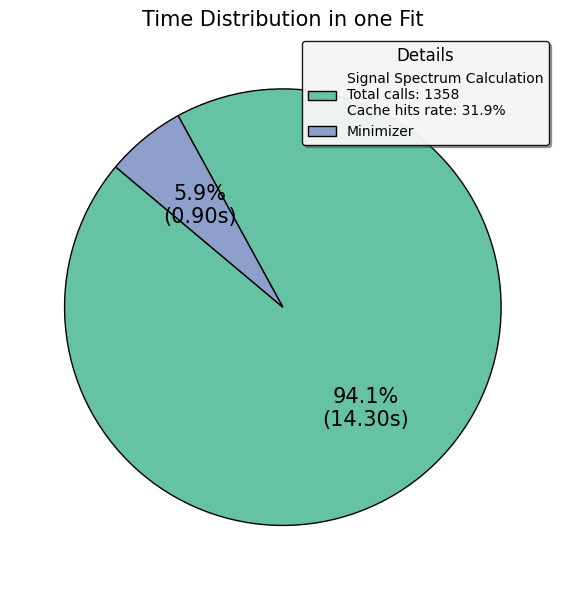
\includegraphics[width=\linewidth]{figure/CNP_fittime.png}
        \caption{CNP $\chi^2$}
        \label{fig:cnp_fittime}
      \end{subfigure}\hfill
      \begin{subfigure}[t]{0.48\textwidth}
        \centering
        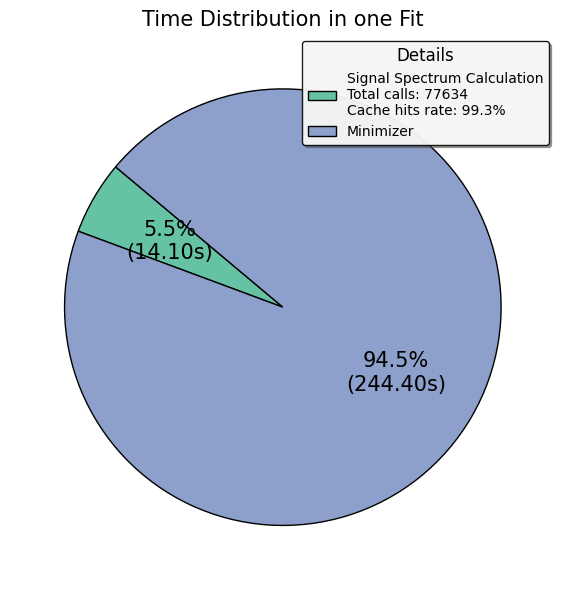
\includegraphics[width=\linewidth]{figure/poisson_fittime.png}
        \caption{Poisson $\chi^2$}
        \label{fig:poisson_fittime}
      \end{subfigure}
    \end{minipage}
  }
  \caption{Time distribution of one full fit after enabling caching for both CNP and Poisson analyses. 
  \textbf{(a) CNP:} the signal–spectrum calculation takes about 14.3\,s (94.1\%), while the minimizer costs about 0.9\,s (5.9\%); the cache hit rate is 31.9\%.
  \textbf{(b) Poisson:} the minimizer dominates the runtime with 244.4\,s (96.3\%), whereas the spectrum calculation contributes only 14.1\,s (5.5\%); the cache hit rate is 94.5\%.}
  \label{fig:fittime_comparison}
\end{figure}




\subsection{CPU and GPU parallelization}
For $\chi^2_{CNP}$, matrix multiplication is the most time consuming part. CPU and GPU parallelization can significantly accelerate matrix multiplication. We use PyTorch to parallelize the heavy matrix multiplications on both CPUs and GPUs. By converting inputs to torch.Tensor, moving them to the target device (.to(cuda) or .to(cpu)) and using torch.matmul/batched ops, PyTorch automatically uses multi-threaded CPU kernels or CUDA to run the work in parallel. This approach is simple to implement and yields substantial speedups with minimal code changes.
By contrast, for the Poisson-likelihood $\chi^2$ statistic, the dominant cost typically lies in the minimizer (many serial function evaluations) rather than in spectrum matrix multiplications; therefore simply parallelizing matrix multiplications yields little overall speedup.
\begin{figure}[htbp]
  \centering
  % 调整 width 或 height 以适配你的版面
  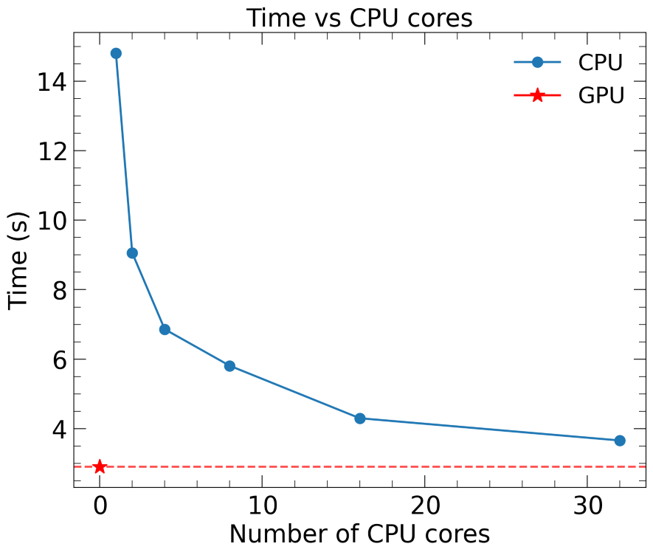
\includegraphics[width=0.35\textwidth]{figure/time_vs_cores.png}
  \caption{Wall-clock time per single fit as a function of the number of available CPU cores, using the CNP (Gaussian-approximate) statistic. The blue curve with markers shows the wall-clock time for one fit when run on CPU with varying numbers of cores; the red star and dashed horizontal line indicate the single-fit time measured on an NVIDIA A30 GPU.}
  \label{fig:time_vs_cores}
\end{figure}

\section{Comparison of fit bias between Poisson and CNP methods}
To evaluate the robustness of the two statistical approaches, we generated a large ensemble of pseudo-experiments and performed a full fit for each pseudo-experiment. The best-fit value from all pseudo-experiments were collected into a histogram to examine whether the estimator exhibits a systematic bias.

Figure~\ref{fig:poisson_vs_cnp} shows that the Poisson-likelihood analysis consistently recovers the true parameter value, whereas the CNP approach exhibits a noticeable shift when some bins contain too few events. If the CNP approximation is used, the bin width should be increased to ensure sufficiently large statistics per bin thereby reducing the resulting bias.

\begin{figure}[htbp]
  \centering
  \begin{subfigure}[t]{0.48\textwidth}
    \centering
    % Replace 'fig_poisson.png' with your Poisson plot filename
    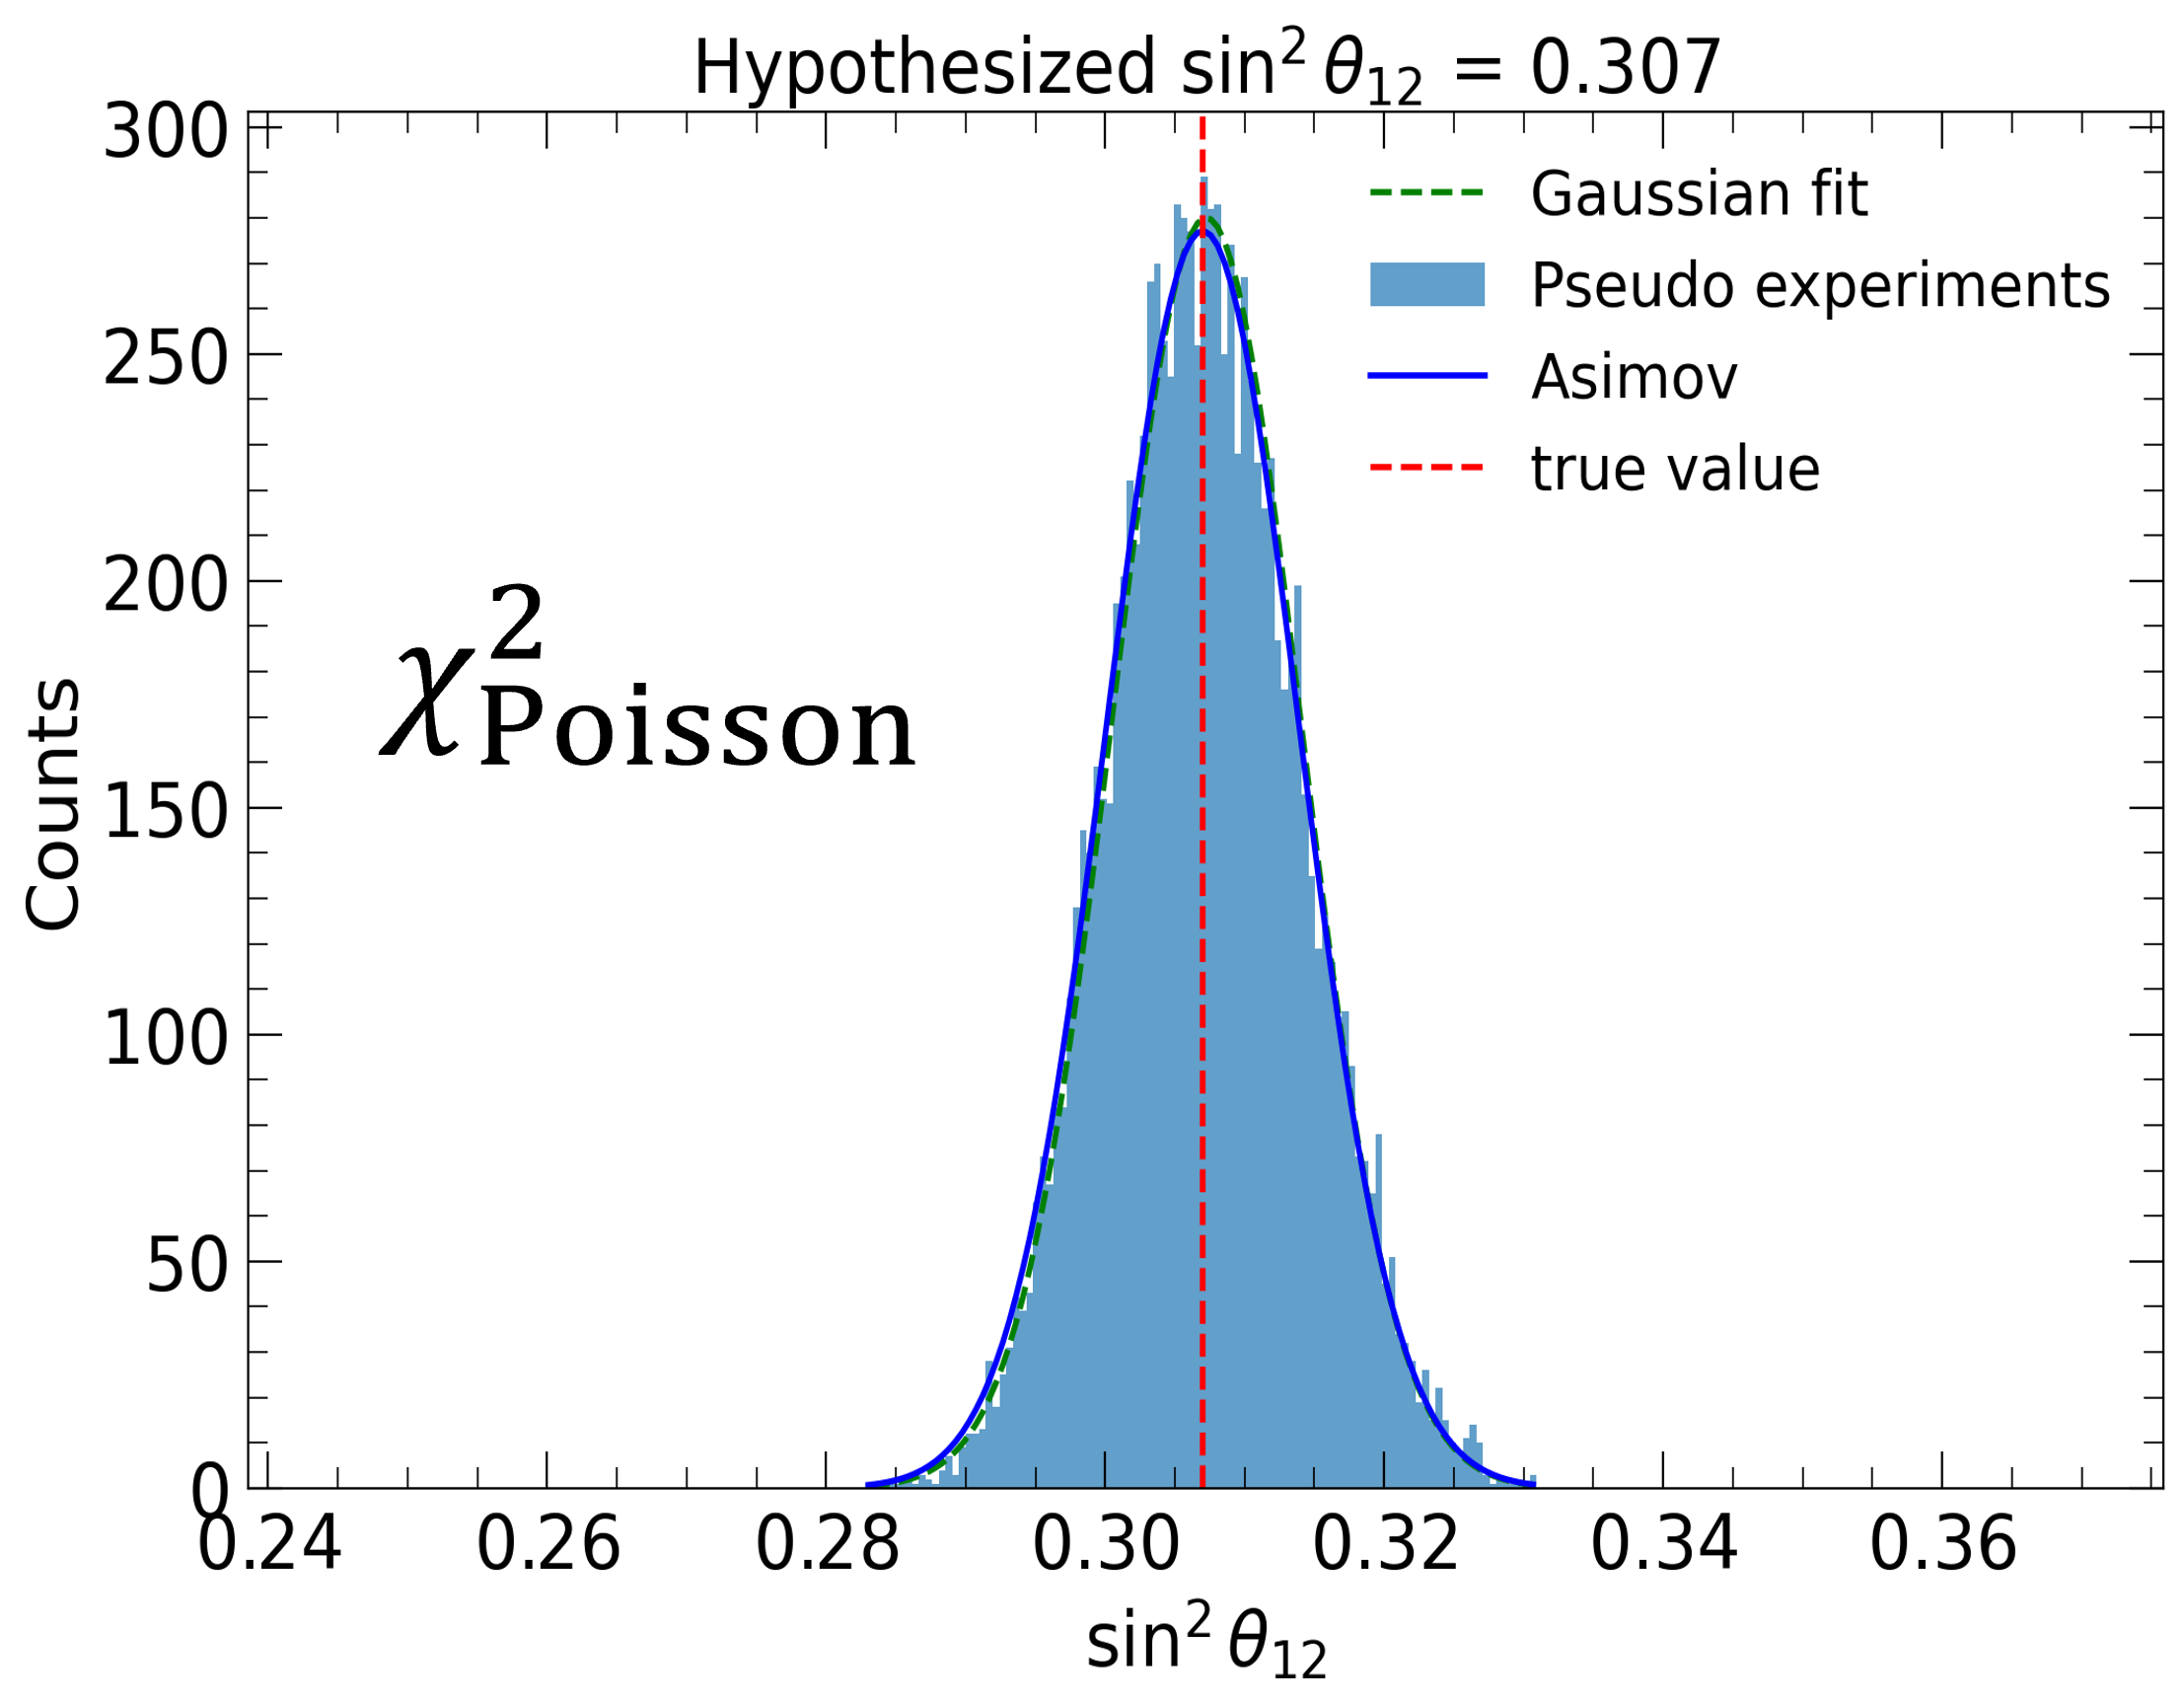
\includegraphics[width=\linewidth, height=5cm]{figure/poisson.png}
    \caption{Distribution of best-fit values from pseudo-experiments using the Poisson likelihood. The blue filled histogram shows the distribution of pseudo-experiment results, the red dashed line marks the true value, and the blue solid line represents the Gaussian fit to the Asimov data.}
    \label{fig:poisson_hist}
  \end{subfigure}\hfill
  \begin{subfigure}[t]{0.48\textwidth}
    \centering
    % Replace 'fig_cnp.png' with your CNP plot filename
    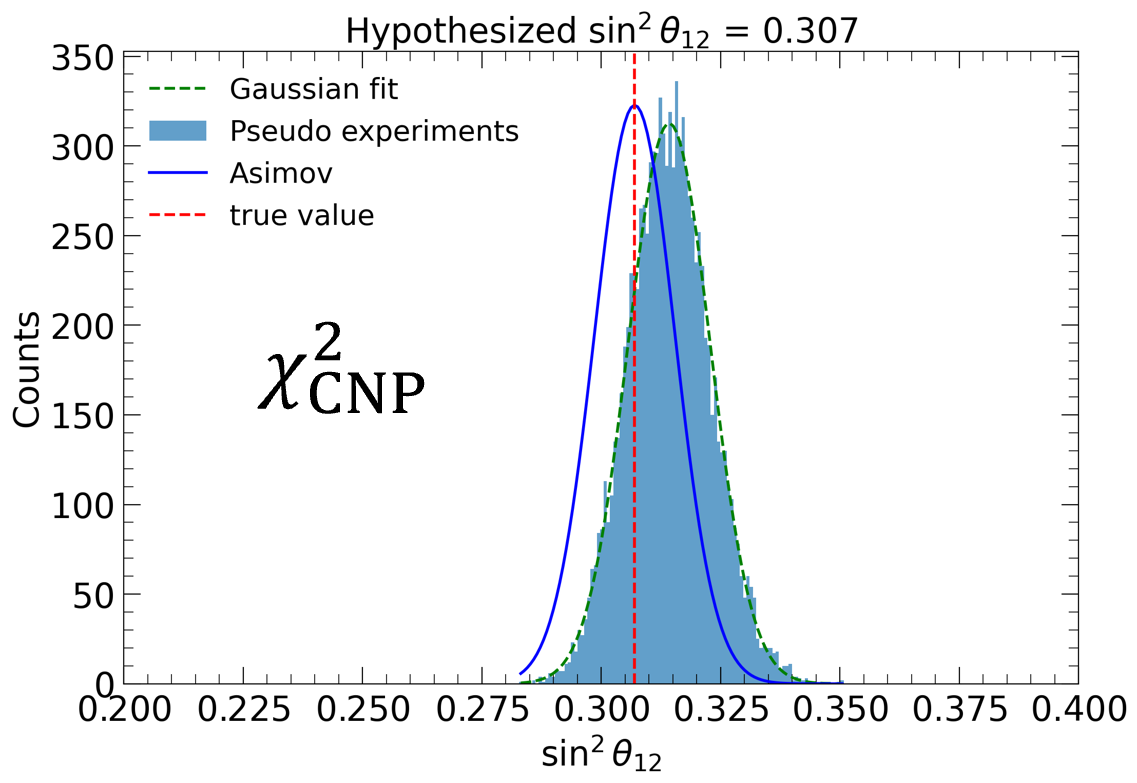
\includegraphics[width=\linewidth, height=5cm]{figure/CNP.png}
    \caption{Same as (a) but for the CNP (Gaussian-approximate) statistic. The distribution shows a systematic shift relative to the true value, indicating bias when some bins have low counts.}
    \label{fig:cnp_hist}
  \end{subfigure}
  \caption{Comparison of fit results obtained from many pseudo-experiments. (a) Poisson-likelihood fits produce an unbiased distribution centered on the true parameter value. (b) CNP (Gaussian-approximate) fits exhibit a bias in the low-statistics regime because the Gaussian approximation is not valid for low counts in some bins. All results are obtained using a uniform binning scheme with a bin width of 20\,keV.}
  \label{fig:poisson_vs_cnp}
\end{figure}

\section{Summary}
Both CNP (Gaussian-approximate) and Poisson-likelihood analyses can be accelerated using function-level caching. In our tests, caching yields roughly a $3\times$ speed-up for CNP-type Gaussian $\chi^2$ fits (cache-hit rate $\approx31.9\%$) and roughly a $6\times$ speed-up for Poisson-likelihood fits (cache-hit rate $\approx99.3\%$). Profiling indicates that, for CNP/Gaussian fits the runtime is dominated by spectrum construction (large matrix multiplications), whereas for Poisson fits the runtime is dominated by minimizer overhead. Using the accelerated fitter, we performed large pseudo-experiment campaigns to study estimator bias: at low statistics, the CNP Gaussian approximation produces a systematic bias because some bins do not satisfy the conditions required for the Gaussian approximation; this bias can be reduced by increasing the bin width, thereby raising the counts per bin. The Poisson-likelihood $\chi^2$ estimator remains unbiased under the same conditions. Therefore, we recommend using the Poisson likelihood for low-count bins; alternatively, one should increase the bin size and validate any CNP-based results with dedicated simulations.



\bibliographystyle{JHEP}
\bibliography{biblio}


\end{document}
